
\documentclass{article}

\usepackage{graphviz}
\usepackage{url}
\usepackage{hyperref}
\usepackage{fullpage}
\usepackage{parskip}
\usepackage{fancyvrb}
\usepackage{amsmath}
\usepackage{framed}

\usepackage{listings}
\lstset{numbers=left,
		basicstyle=\footnotesize,
		captionpos=b,
		xleftmargin=0.3in}

\providecommand{\e}[1]{\ensuremath{\times 10^{#1}}}

\VerbatimFootnotes

\raggedright

% Change enumerate section numbering
\renewcommand*{\theenumii}{\theenumi.\arabic{enumii}}
\renewcommand*{\labelenumii}{\theenumi.\arabic{enumii}}

\begin{document}

% {{{ title page
\vspace*{1.0in}

\centerline{\LARGE \textbf{SprinklerPI}}
%\centerline{(Product Test Plan)}
\vspace{0.3in}
\centerline{\LARGE Product Test Plan}

\vfill

\begin{center}
\begin{tabular}{c}
Jeremiah Mahler \\
EECE 490B, CSU Chico \\
\today
\end{tabular}
\end{center}

\vspace{1in}

\thispagestyle{empty}

%\vfill

\pagebreak
% }}}

\thispagestyle{empty}
\tableofcontents
\clearpage

% {{{ Information Required for Execution
\section{Information Required for Execution}

\subsection{Purpose}

The purpose of this test protocol is to verify the full and complete
operation of the SprinklerPI system.

\subsection{Scope}

This test protocol should be executed to verify that each principal feature
and function performs within specification called out by the engineering
requirements document. In addition, other necessary specifications shall
be tested such as specific and necessary user, installation and power
requirements. The testing called out in this protocol is subject exclusively
to those selected specifications provided for the SprinklerPI.

\subsection{Responsibilities}

It is the responsibility of the assigned test engineer to execute all tests
included herein to the best of their ability. If necessary, seek additional
assistance to execute tasks.

\subsection{References}

Not applicable at this time.

%\subsection{Definitions}

\subsection{Equipment/Supplies}

\begin{itemize}
\item 110 volts AC power supply.
\item Digital volt meter.
\item Three test bridges (25 $\Omega$, 50 watt).
\item Ethernet network connection.
\item (optional) Wireless usb adapter.
\end{itemize}

\subsection{Precautions \& Warnings}

This test plan contains certain warnings, cautions and important
notes that the test engineer must be aware of while performing these tests.
The following illustrates each of these messages and how to recognize them.

\fbox{
\textbf{WARNING: \textless message\textgreater}
}

The ``WARNING: Message'' alerts the user about safety issues that are of
the highest importance, such as possible injury to the operator.

\fbox{
\textbf{CAUTION: \textless message\textgreater}
}

The ``CAUTION: Message'' alerts the user to issues concerning possible
damage to the equipment or that can lead to erroneous test results.

\fbox{
\textbf{IMPORTANT: \textless message\textgreater}
}

The ``IMPORTANT: Message'' alerts the user to important design changes.

% }}}

% {{{ Testing Features and Functions
\section{Testing Features and Functions}

This testing procedure can be used to determine if the system
is fully functional and operating within acceptable tolerances.

This is a minimal set of tests done at a high level of abstraction.
Low level sub-tests which provide no useful increase in the test scope
are not included.
In the event that a fault is found it is left up to an engineer to
determine the root cause.

Several assumptions are made in this test procedure.
It is assumed that networking has already been configured as
described in Appendix \ref{app:networking}.
It is also assumed that a fully populated SprinklerPI system with
three control/drivers is being tested.
This system is modular and the number of control/drivers can vary
from one to three.
Adapting these procedures to a reduced number of control/drivers should
be straightforward but this reduces the scope of the tests.

% {{{ Power On Test
\subsection{Power On Test}

\begin{enumerate}
\item Equipment Required
	\begin{itemize}
		\item 110 volts AC power outlet (NEMA 5-15R).
	\end{itemize}
\item Input
	\begin{itemize}
	\item (none)
	\end{itemize}
\item Output
	\begin{itemize}
	\item Green power LED on.
	\item Activity LEDs during boot up.
	\item Control LEDs off.
	\end{itemize}
\item Test Description \\

During power up the system should be seen going through several states
which can be seen by observing LED indicators (Figure \ref{fig:ledind}).
When it is complete it should end in a specific state.

After plugging the cord in to a 110 volt AC outlet the green LED on
the power supply should go on.
Then, as the computer boots up, activity should be seen on its LEDs.
The control LEDs may go on/off randomly as the system boots.
They also may may turn on valve number one during boot.
This is normal as the output pins go through random states and
is eventually cleared.
After approximately 30 seconds the activity LEDs on the computer
should reduce which indicates that the system has completed booting.
At this point all control/driver LEDs should be off.

\begin{figure}[hbp!]
% TODO - picture of fully populated system.
%      - label each of the LED indicators.
\caption{Location of LED indicators.}\label{fig:ledind}
\end{figure}

\pagebreak
\item Test Results \\
\vspace{1em}
\begin{tabular}{|l|l|l|l|}
	\hline
	\multicolumn{1}{|c|}{Test}
	& \multicolumn{1}{|c|}{Value}
	& \multicolumn{1}{|c|}{Pass/Fail}
	& \multicolumn{1}{|c|}{Notes} \\
	\hline
	Power LED on? & on / off && \hspace{1.7in} \\
	\hline
	Activity LEDs during boot? & yes / no && \\
	\hline
	Stable activity LEDs after boot up? & yes / no && \\
	\hline
	Control outputs off after boot up? & yes / no && \\
	\hline
\end{tabular}

\end{enumerate}
% }}}

% {{{ Manual Control Test
\clearpage
\subsection{Manual Control Test}

\begin{enumerate}
\item Equipment Required
	\begin{itemize}
	\item 110 volts AC power outlet (NEMA 5-15R).
	\item PC with Internet access and a web browser.
	\end{itemize}
\item Input
	\begin{itemize}
	\item User turns valves on using manual mode of web interface.
	\end{itemize}
\item Output
	\begin{itemize}
	\item LED indicator for each valve which is turned on.
	\end{itemize}
\item Test Description \\

These tests verify that the valves can be manually operated from
the web interface (Figure \ref{fig:www-manual_mode}).
The user iterates through each possible combination and verifies
that the LED valve indicator is correct.

\begin{figure}[hbp!]
\begin{center}
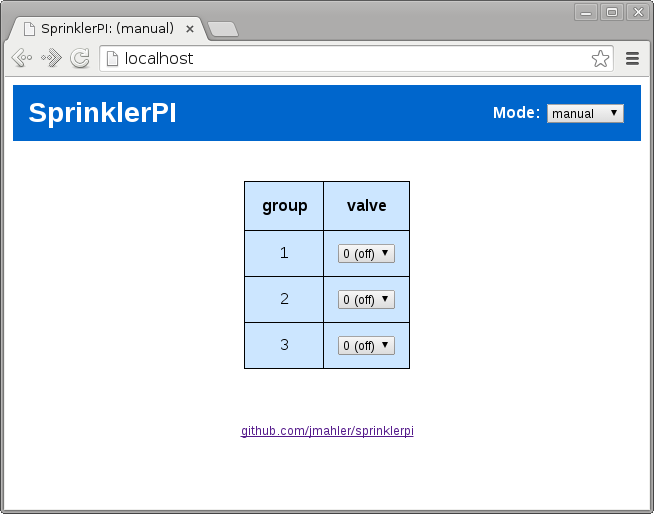
\includegraphics[scale=0.5]{img/www-manual_mode}
\end{center}
\caption{Web interface in manual mode which allows operation of
a single valve for each group.
The URL may be different depending on how the network is configured.}
\label{fig:www-manual_mode}
\end{figure}

It is assumed network has already been configured
(Appendix \ref{app:networking}) and that the URL of the server being
used for testing is known.

\pagebreak
\item Test Results \\
	\vspace{1em}
	\begin{tabular}{|c|c|c|c|c|}
		\hline
		Group & Valve & Value & Pass/Fail & Notes \\
		\hline
		1 & 1 & on / off && \hspace{20em} \\
		\hline
		1 & 2 & on / off && \\
		\hline
		1 & 3 & on / off && \\
		\hline
		1 & 4 & on / off && \\
		\hline
		1 & 5 & on / off && \\
		\hline
		1 & 6 & on / off && \\
		\hline
		1 & 7 & on / off && \\
		\hline
		1 & 8 & on / off && \\
		\hline
		\hline
		2 & 1 & on / off && \\
		\hline
		2 & 2 & on / off && \\
		\hline
		2 & 3 & on / off && \\
		\hline
		2 & 4 & on / off && \\
		\hline
		2 & 5 & on / off && \\
		\hline
		2 & 6 & on / off && \\
		\hline
		2 & 7 & on / off && \\
		\hline
		2 & 8 & on / off && \\
		\hline
		\hline
		3 & 1 & on / off && \\
		\hline
		3 & 2 & on / off && \\
		\hline
		3 & 3 & on / off && \\
		\hline
		3 & 4 & on / off && \\
		\hline
		3 & 5 & on / off && \\
		\hline
		3 & 6 & on / off && \\
		\hline
		3 & 7 & on / off && \\
		\hline
		3 & 8 & on / off && \\
		\hline
	\end{tabular}
\end{enumerate}
% }}}

% {{{ Load Test  XXX TODO
\clearpage
\subsection{Load Test}

\begin{figure}[htbp!]
\begin{center}
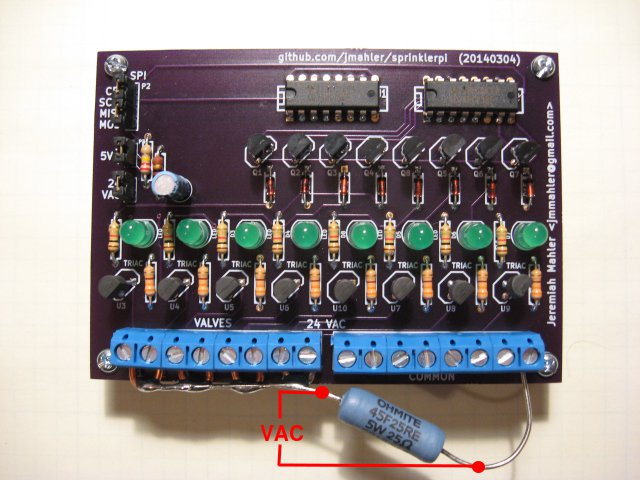
\includegraphics[scale=0.6]{img/control_driver_tb_03.jpg}
\end{center}
\caption{Voltage test point for control driver test bridge.}\label{fig:cdbtest}
\end{figure}

\begin{figure}[htbp!]
\begin{center}
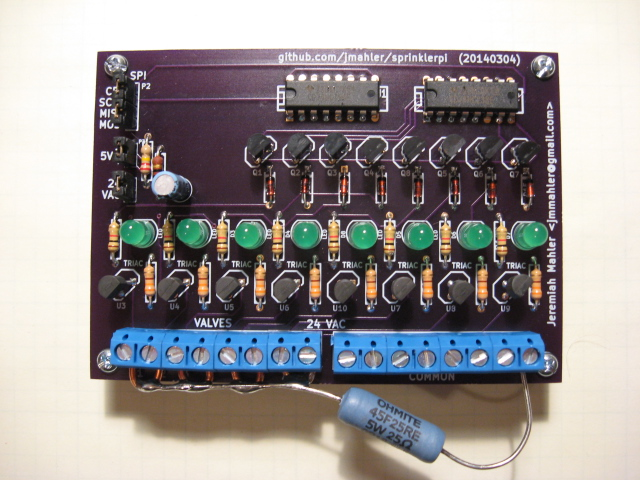
\includegraphics[scale=0.6]{img/control_driver_tb_02.jpg}
\end{center}
\caption{Control driver with test bridge (bottom) installed.}
\label{fig:cdbridge}
\end{figure}


\begin{framed}
\textbf{IMPORTANT}: The DC voltage output of the power supply has
been changed from 5V to 3.3V.
The label on version 20140304 of the power supply PCB still
refers to 5V despite this change.
\end{framed}

\begin{figure}[hbp!]
\begin{center}
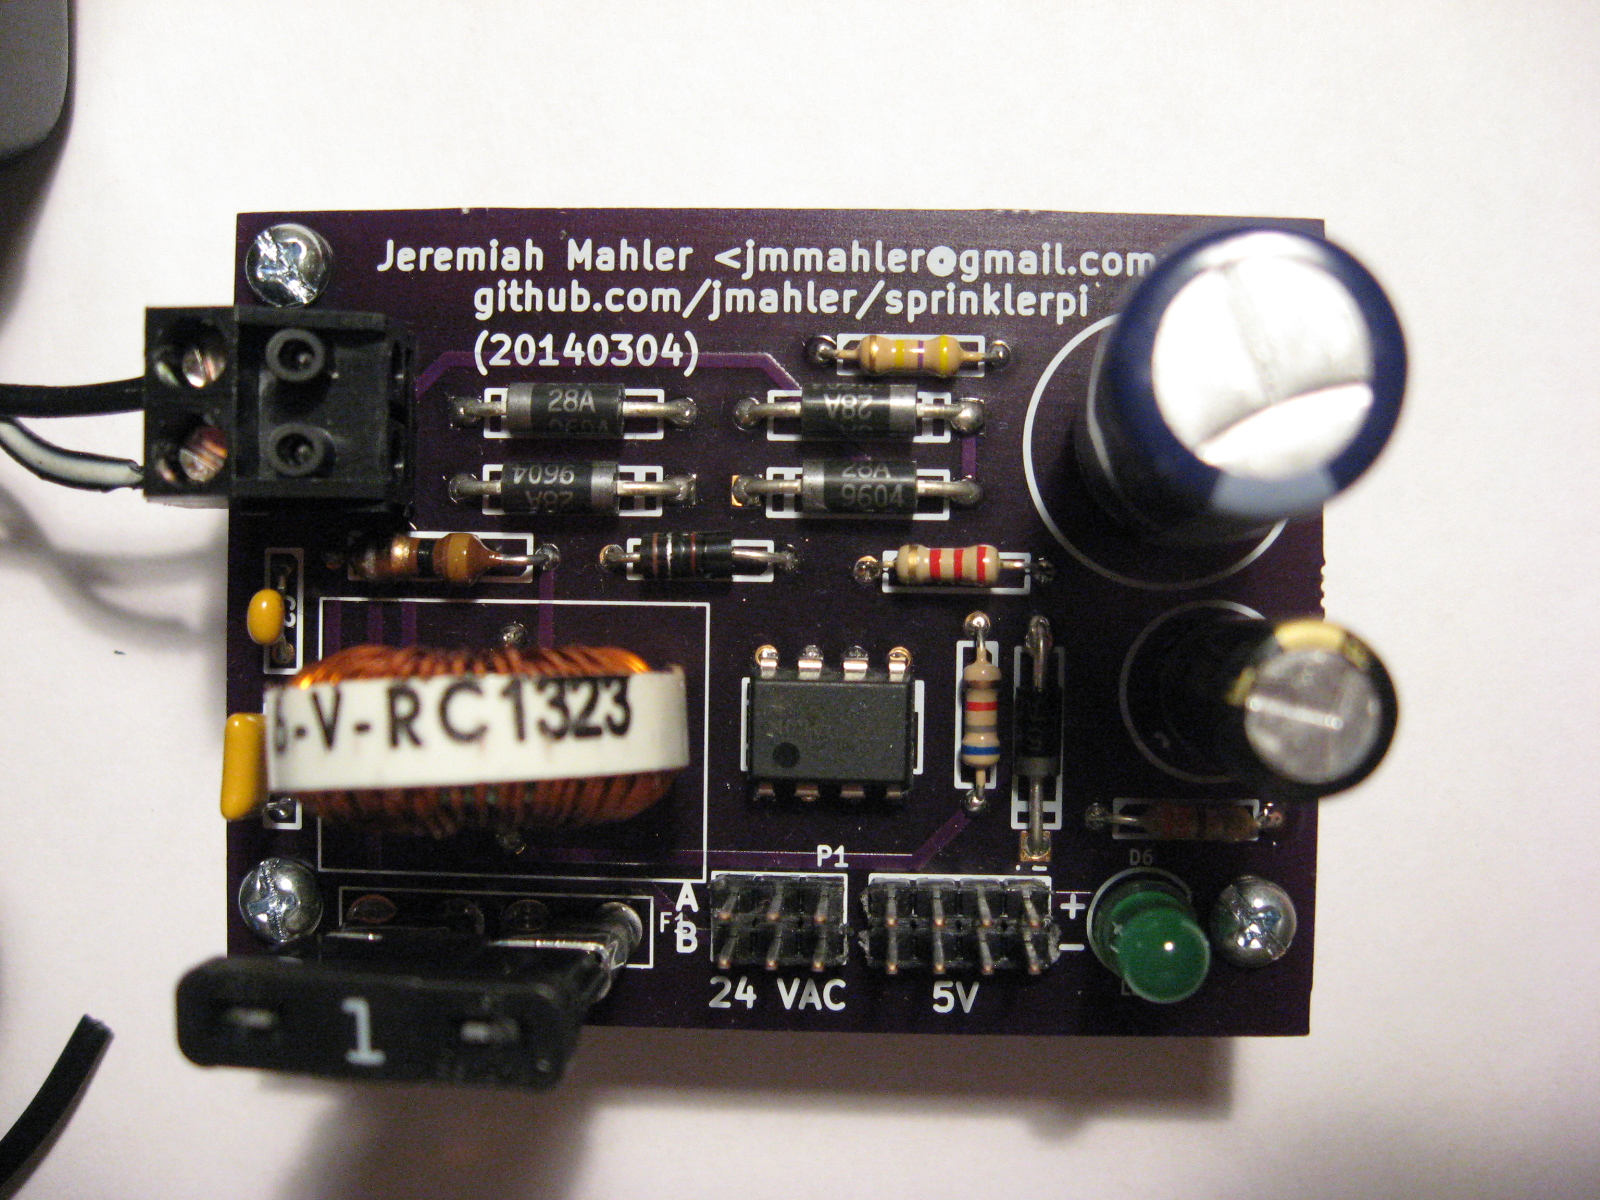
\includegraphics[scale=0.15,angle=0]{img/power_pcb-assembled-02.jpg}
\end{center}
\caption{Assembled power supply module PCB.
The 24 volts AC input is in the top left.
The green power LED is on the bottom right.
The headers for 24 volts AC output and 3.3 volts DC
output are on the bottom.
}\label{fig:psm2}
\end{figure}

\begin{enumerate}
\item Equipment Required
	\begin{itemize}
	\item SprinklerPI power supply module (revision 20140304).
	\item 110 volts AC power supply (standard U.S.).
	\item 110 volts AC to 24 volts AC power adapter.
	\item Digital multi meter.
	\item Control/Driver test bridge (25 $\Omega$, 5 Watt)
			(Figure \ref{fig:cdbridge}).
	\end{itemize}
\item Input
	\begin{itemize}
	\item 24 volts AC from 110 to 24 volts AC adapter.
	\end{itemize}
\item Output
	\begin{itemize}
	\item $9.5\pm0.5$ volts AC across test bridge resistor when on.
	\item Green power LED on.
	\item 24$\pm4.8$ (20\%) volts AC output.
	\item 3.3$\pm0.3$ (10\%) volts DC output.
	\end{itemize}
\pagebreak
\item Test Description \\

The 110 volt to 24 volt AC power adapter should be connected to the
two pin input header (Figure \ref{fig:psm2}, top left) and screwed down.
With the power adapter plugged in to a 110 volts AC power supply the
green power LED should come on.
Using a DMM to measure voltage, there should be 3.3 volts DC output on
the ``5V'' header pins and 24 volts AC output on the ``24 VAC'' header pins.
Be sure to switch from AC to DC modes on the DMM as necessary.
The polarity of DC voltages are denoted on the PCB (Figure \ref{fig:psm2}).

\item Test Results \\
	\vspace{0.2in}
	\begin{tabular}{|l|l|l|l|}
		\hline
		& Value & Pass/Fail & Results/Data\hspace{2in} \\
		\hline
		Power LED on? &&& \\
		\hline
		$24\pm4.8$ volts AC &&& \\
		\hline
		$3.3\pm0.3$ volts DC &&& \\
		\hline
	\end{tabular}

\item Test Results \\
	\vspace{1em}
	\begin{tabular}{|l|l|l|l|l|}
		\hline
		& LED on? & Voltage Drop    & Pass/Fail & Results/Data\hspace{2in} \\
		&         & $9.5\pm0.5$ VAC & & \\
		\hline
		1 &&&& \\
		\hline
		2 &&&& \\
		\hline
		3 &&&& \\
		\hline
		4 &&&& \\
		\hline
		5 &&&& \\
		\hline
		6 &&&& \\
		\hline
		7 &&&& \\
		\hline
		8 &&&& \\
		\hline
	\end{tabular}

\end{enumerate}
% }}}

% {{{ Scheduling Test

% }}}

%\section{Other Testing}

% {{{ User Interface
\clearpage
\subsection{User Interface}

\begin{enumerate}
\item Equipment Required
	\begin{itemize}
	\item Computer with web browser and network connection.
	\end{itemize}
\item Input
	\begin{itemize}
	\item Turn valve on/off.
	\item Check status of valve.
	\item Schedule time and duration to run valve.
	\end{itemize}
\item Output
	\begin{itemize}
	\item Valves go on when commanded.
	\item Status of operating valve shown when on.
	\item Scheduling a time and duration works as expected.
	\item Pass: Valves operate according to the commands.
	\item Fail: Response is not expected.
	\end{itemize}
\item Test Description \\

The basic commands given through the web interface are:
on/off valve, show current status, schedule a time/duration.
These tests verify these operations.

\item Test Results \\
	\vspace{0.25in}
	\begin{tabular}{|l|l|l|l|l|l|c|}
		\hline
		\multicolumn{7}{|c|}{Valves On/Off} \\
		\hline
		\# & On? & On Status? & Off? & Off Status? & Pass/Fail & \hspace{0.7in}Notes\hspace{0.7in} \\
		\hline
		1 &&&&&& \\
		\hline
		2 &&&&&& \\
		\hline
		3 &&&&&& \\
		\hline
		4 &&&&&& \\
		\hline
		5 &&&&&& \\
		\hline
		6 &&&&&& \\
		\hline
		7 &&&&&& \\
		\hline
		8 &&&&&& \\
		\hline
	\end{tabular}

	\vspace{0.25in}
	\begin{tabular}{|l|l|l|l|l|}
		\hline
		\multicolumn{5}{|c|}{Schedule} \\
		\hline
		\# & Time Start & Time End & Pass/Fail & \hspace{0.5in}Notes\hspace{0.5in} \\
		\hline
		& now & now + 1 minute & & \\
		\hline
		& now & now + 5 minute & & \\
		\hline
	\end{tabular}

\end{enumerate}

% }}}

% }}}

\clearpage
\appendix

% {{{ Network Configuration
\section{Network Configuration}
\label{app:networking}

% TODO

% }}}

\end{document}

